
\documentclass{article}

\usepackage[top=3cm, bottom=3cm, left=3cm, right=3cm]{geometry}

\usepackage[french]{babel}
\usepackage[utf8]{inputenc}
\usepackage[T1]{fontenc}

\usepackage{pdfpages}

\usepackage{graphicx}
\usepackage{caption}

\usepackage{tikz}
\usetikzlibrary{positioning,shapes,arrows,automata}
\tikzset{>=stealth'}

\title{Proposition de projet : TriComp}

\author{}

\date{29 Septembre 2014}

\begin{document}

\makeatletter % Pour utiliser le "at" comme une commande interne.
  \begin{titlepage}
    \begin{center}
       {\LARGE \@title} \\
       \vspace{1cm}
       {\large \@date}
       \vspace{2cm}
    \end{center}
       {\large
       William \textsc{Aufort} \hfill Julien \textsc{Bensmail}, coordinateur\\
       Agathe \textsc{Herrou}  \hfill Romain \textsc{Labolle} \\
       Frédéric \textsc{Lang} \hfill Maxime \textsc{Lesourd} \\
       Laureline \textsc{Pinault} \hfill Léo \textsc{Stéfanesco}}
  \tableofcontents
  \end{titlepage}
\makeatother

\pagebreak

% Esquisse de plan ( proposee ) bis :
%
% I] Introduction et objectifs
% II] Produits concurrents
% III] Cahier des charges et applications
%     a) Fonctionnalités :
%     b) Aspects techniques : les différents modules (gui, compilation, lg haut niveau,...) + diagrammes
%     c) public vise et retombees attendues
%     d) Améliorations possible
% IV] Organisation du projet
%     a) Description de l'equipe : (nombre/nom/prenom des collaborateurs, affinités/compétences variées...) + moyen de communication,.. au sein de l'équipe (git, pad, réunions, ...)
%     b) Workpackages
%     c) Les différentes phases : Modèle par couches (versions successives)
%     d) Calendrier des taches



\section{Introduction et objectifs}

Le tricot est une technique utilisée pour créer une étoffe à partir de fils. Ses origines remontent au $X^{eme}$ siècle.
Redevenu à la mode dans toutes les tranches d'âge, il a aussi connu un développement au travers de l'informatique. Il existe en effet
quelques logiciels relatifs au tricot, mais ceux-ci visent un public plutôt expert, que ce soit en tricot ou en informatique (comment
décrire un tricot à l'ordinateur ?).

Le projet TriComp visait au départ à concevoir un Compilateur pour Tricot (d'où son nom) afin de faciliter davantage l'interaction entre
tricoteur et machine. Après un examen de l'état de l'art, nous avons davantage ciblé nos objectifs. Notre objectif principal est de
fournir un logiciel disposant de fonctionnalités à la fois de création (de modèles), de visualisation et de conception (tricot),
destiné au plus grand nombre (c'est-à-dire sans connaissances poussées en informatique et en tricot).

Ce document présente notre proposition de projet. Après avoir détaillé l'état de l'art des logiciels de tricot existants, nous exposerons
notre cahier des charges et nos objectifs dans le détail. Enfin, nous détaillerons le déroulement du projet, à savoir les différents
workpackages identifiés ainsi qu'un calendrier rassemblant les différentes tâches.


\section{Produits concurrents}



\subsection{OpenKnit}

OpenKnit est une machine qui permet à ses utilisateurs de concevoir des vêtements en entrant leurs instructions dans un contrôleur Arduino
(un circuit intégré). Même si l'utilisateur peut créer ou télécharger des modèles, ce projet comporte une grande part de hardware, et est
plutôt orienté vers la fabrication du produit que sa conception (les instructions sont directement transmises à la machine OpenKnit). Il
est donc plutôt destiné à un public qui souhaite faire fabriquer de simples créations et non pas aux tricoteurs (ce qui n'enlève rien au
caractère innovant de ce projet).

\subsection{DesignaKnit}

DesignaKnit est un logiciel permettant de créer des modèles de tricot destinés à être réalisés à la main ou avec une machine à tricoter.
Destiné plutôt à un public confirmé, celui-ci est assez complet propose quelques outils innovants, comme un convertisseur d'images vers un
motif réalisable en tricot.

\subsection{KP}

KP est un langage bas niveau développé en 2004 pour aider les tricoteurs à écrire des modèles de tricot. Il offre la possibilité de
combiner ou d'ajuster des modèles pour en créer de nouveaux. Ce langage est accompagné d'un interpréteur qui génère des instructions elles
aussi bas niveau. Bien qu'il fut abandonné avant d'être aboutit, ce projet peut représenter un départ intéressant dans notre phase de conception de
nos langages.

\subsection{KnitML}

Le projet KnitML a également pour but de fournir un langage bas niveau au service des tricoteurs et développeurs de logiciels lié au
tricot. Par exemple, le logiciel Knitter se base sur KnitML pour fournir une visualisation 3D du modèle passé en entrée. Il est davantage
actualisé (la dernière version date de 2012) et peut également nous apporter une précieuse aide.

\subsection{Les solutions industrielles ?} Peut être se renseigner ?

\section{Cahier des charges et applications}

\subsection{Fonctionnalités}

\subsection{Aspects techniques}


\subsubsection{Formalisation d'un langage}

La description d'un langage pour décrire les tricots ainsi que sa formalisation est un objectif primordiale.
Une telle description se fera par une formation continue en tricot, qui permettra d'ajouter de nouveaux points (i.e de nouvelles
possibilités pour le tricot) tout au long du projet, mais également d'avoir une vue plus générale sur la manière de concevoir un tel
langage. La formalisation du langage résultant sera également un objectif clé de ce projet.

\subsubsection{Compilation}

C'est l'intitulé du projet : construire un compilateur pour tricot. Le compilateur aura pour rôle de transformer le tricot que
l'utilisateur souhaite créer en une interprétation dans un langage bas niveau (type KP), qui pourra ensuite être traduit en une succession
d'instructions que celui-ci pourra réaliser.
Le compilateur devra également être capable de détecter des impossibilités au niveau de la conception du modèle.

La conception du compilateur présuppose également d'avoir défini (tout comme nous aurons défini le langage de la section précédente) un
langage pour les instructions qui seront générées (un peu comme dans un manuel de tricot).
Une fois ce langage défini, nous pourrons nous concentrer sur la phase de conception du compilateur.

\subsubsection{Réalisation logicielle : interface pour tricoteur}

Notre réalisation logicielle a pour but de mettre le compilateur précédent au service des utilisateurs.

L'objectif ici est de concevoir un logiciel fournissant à ses utilisateurs essentiellement deux fonctionnalités :
\begin{itemize}
  \item \textbf{La conception d'un tricot via une interface graphique} Notre objectif ici est de mettre en place pour l'utilisateur des
  outils afin qu'il puisse entrer son projet de tricot : choix d'un modèle (pull, écharpe...), choix des points utilisés
  (jersey, ...), de la couleur.
  \item \textbf{Le suivi personnalisé} Une fois que l'utilisateur aura saisi son tricot, le logiciel appellera le compilateur afin de générer
la liste des instructions qui devront être suivies pour réaliser le tricot. Ces instructions permettront un suivi du tricoteur par le
logiciel : le tricoteur pourra à travers le logiciel suivre les différentes étapes, avec notamment des illustrations de la tâche à
accomplir et l'observation du résultat à obtenir à chaque étape.
\end{itemize}

\subsubsection{Diagramme des interactions}

    Voir Figure \ref{diag-composants}.

    \begin{figure}[!h]
    \centering

    \begin{tikzpicture}[->,>=stealth',shorten >=1pt,auto,node distance= 3.5cm,
                    semithick]
      \tikzstyle{every state}=[draw=black,text=black]

      \node[state]     (user)   []                                  	  {Utilisateur};
      \node[state]     (gui)	[]                [right of=user]     	  {GUI};
      \node[state]     (HN) 	[shape=rectangle] [above right of=gui]    {Langage haut niveau};
      \node[state]     (compil) []                [right of=HN]       	  {Compilateur};
      \node[state]     (BN)     [shape=rectangle] [below right of=compil] {Langage bas niveau};
      \node[state]     (trad)   []                [below left of=BN]  	  {Traducteur};
      \node[state]     (manuel) [shape=rectangle] [left of=trad]    	  {Instructions};
      \node[state]     (machine)[dashed] [below of=BN] {\textit{Machine}};


      \path (user)   edge               node {Spécifications} (gui)
		     edge [bend left=15]node{}		(HN.west)
        (gui)        edge [bend left]   node {}               (HN.west)
        (HN.south)   edge               node {Visualisation}  (gui)
        (HN)         edge               node {}               (compil)
        (compil)     edge               node {}               (BN)
        (BN)         edge          	node {}               (trad)
		     edge [dashed] 	node {}		 (machine)
        (trad)       edge          	node {}               (manuel)
        (manuel)     edge               node {Affichage}      (gui)
        ;
    \end{tikzpicture}

    \caption{Interaction entre les différents composants}
    \label{diag-composants}
    \end{figure}

\subsection{Motivations}

\subsection{Public visé et retombées attendues}


Comme dit précédemment, notre projet vise tous les tricoteurs, experts ou non, recherchant un assistant dans la conception et la
réalisation de leurs oeuvres.

\subsection{Améliorations possibles}

\section{Organisation et planification}

\subsection{L'équipe}

L'équipe de notre projet TriComp comporte sept étudiants de M1 ainsi qu'un coordinateur
% Redonner les noms ici ?

\subsection{Les différentes phases}

Nous avons prévu de développer 3 versions de notre logiciel. Chaque version sera basée sur la précédente et incluera de nouvelles fonctionnalités notamment au niveau de la variété des points proposés.
Les phases du projet correspondent aux différentes versions que nous avons prévu de réaliser.

% Ici descriptifs de ce qu'il y aura ds les différentes version, agathe ?

\subsection{Workpackages}

Nous avons divisé le travail à effectuer en worpackages, correspondant globalement aux différents composants du logiciel. Ces workpackages eux-même sont subdivisés en tâches.

Ci-dessous le détail et la répartition humaine des tâches (la personne en gras est responsable du bon déroulement de la tâche) :

\begin{description}
\item[WP 1 : Langage bas niveau] Ce workpackage est destiné à concevoir les instructions du langage bas niveau et ce qui tourne autour. Les tâches de ce workpackages sont les suivantes :

    \begin{description}
    \item[Définition du langage] Consiste à définir les instructions du langages.

      \textit{Production : Une liste d'instruction décrivant le langage bas niveau.}

      \textbf{Laureline}

    \item[Module de traduction] Consiste à implémenter un traducteur qui traduira les instructions du langage bas-niveau en des instructions en langage naturel, type manuel de tricot, compréhensible pour l'utilisateur.

      \textit{Production : Un module traduisant le langage bas niveau en instructions de tricot compréhensibles pour l'utilisateur.}

      \textbf{Laureline}
    \end{description}

\medskip

\item[WP 2 : Vérification] A partir de la version 3, le logiciel permettra à l'utilisateur de définir des motifs par combinaisons de points. Or si ces motifs sont définis sans faire attention, il peut y avoir des conflits. Le module de vérification sert à repérer ces conflits lors de la compilation ainsi qu'à indiquer à l'utilisateur où et pourquoi ils ont lieu. Les tâches de ce workpackages sont les suivantes :

    \begin{description}
    \item[Définition des contraintes] Consiste à définir les conflits qui peuvent apparaître.
      
      \textit{Production : Une liste de contraintes décrivant les conflits possibles.}

      \textbf{?}, Léo, Laureline

    \item[Implémentation des contraintes] Consiste à implémenter un module de vérification qui se lancera avec la compilation pour rattraper les erreurs survenant lors de la compilation.
      
      \textit{Production : Un module rattrapant les erreurs liées aux conflits lors de la compilation.}

      \textbf{?}, Léo, Laureline

    \end{description}

\medskip

\item[WP 3 : Compilateur] C'est le coeur du projet : le module qui va traduire le langage haut niveau décrivant le tricot en instruction bas niveau, permettant de réaliser le tricot maille par maille. Ce workpackage est subdivisé en trois tâches semblables, une pour chaque version :

    \begin{description}
    \item[Compilation v.i] A chaque version, le langage au niveau sera étendu, d'où la nécessité de mettre à jour le compilateur pour qu'il prenne en compte les nouveaux éléments du langage. Cette tâche consiste à implémenter un compilateur transformant le langage haut niveau v.i en instructions bas niveau.

      \textit{Production : Un module compilant le langage haut niveau v.i vers des instructions bas niveau.}

      \textbf{?}, Léo, Laureline %respo et équipe à définir selon i ?
    \end{description}

\medskip

\item[WP 4 : Interface graphique] L'interface graphique sera le lien entre l'utilisateur et le logiciel. Elle doit permettre à l'utilisateur un accès ergonomique à toutes les fonctionnalités du logiciel. Elle va également permettre à l'utilisateur de visualiser ce qu'il spécifie et va lui servir d'assistant pour tricoter à partir des instructions fournies. Les tâches de ce workpackage sont les suivantes :

  \begin{description}
  \item[Mise en place de l'interface] Créer l'interface vide, la coquille. Commencer à travailler sur la visualisation.

    \textit{Production : Une interface graphique, pas encore reliée au logiciel}

    \textbf{William}

  \item[Visualisation v.i] Implémenter un module permettant, à partir d'une description en langage haut niveau (version v.i), visualiser l'objet décrit.

    \textit{Production : Un module de visualisation pour le langage haut niveau v.i}

    \textbf{William}, Léo %respo et équipe à définir selon i ?

  \item[Traduction des spécifications v.i] Développer dans l'interface un moyen ergonomique permettant à l'utilisateur d'entrer ses spécifications, lesquelles seront traduites en langage haut niveau (version v.i).

    \textit{Production : Une interface graphique cohérente avec la description i du langage haut niveau, permettant à l'utilisateur de décrire de manière simple et intuitive ce qu'il veut tricoter.}

    \textbf{?}
  \end{description}

\medskip

\item[WP 5 : Langage haut niveau] Ce workpackage est destiné à définir le langage haut niveau permettant de décrire les objets à tricoter.

  \begin{description}
  \item[Définition du langage v.i] Définir un langage permettant de décrire le tricot, avec les fonctionnalités et la variation de points disponibles définies dans les spécifications de la version v.i.

    \textit{Production : Un langage descriptif, étendu à chaque version.}

    \textbf{?}, Léo
  \end{description}

\medskip

\item[WP 6 : Communication] Ce workpackage inclue tout ce qui concerne la communication autour du projet, que ce soit au niveau large public (website), au niveau utilisateur (readme et manuel) ou au niveau compte-rendu de projet (proposal, mid term rapport et final rapport).

  \begin{description}
  \item[Proposal] Rédiger la proposal.

    \textit{Production : Proposal}

    \textbf{Laureline}, William, Léo

  \item[Mid-term Rapport] Rédiger le rapport de mi-projet. Celui-ci contiendra tout le travail réalisé jusque là, et notament le descriptif de la version 1 qui devrait être fonctionnelle d'ici là.

    \textit{Production : Mid-term rapport}

    \textbf{William}, Laureline, Léo

  \item[Final Rapport et présentation] Rédiger le rapport de fin de projet et préparer la présentation du projet.

    \textit{Production : Final rapport et slides de la présentation.}

    \textbf{?}, William, Léo, Laureline, Romain, Maxime, Agathe, Frédéric

  \item[Website] Créer un website pour le projet. %décrire un peu plus

    \textit{Production : Website}

    \textbf{Laureline}

  \item[Readme, Manuel et Website v.i] Mettre à jour le readme, le manuel et le website pour qu'ils soient cohérent avec la version v.i du logiciel.

    \textit{Production : Readme, manuel et website}

    \textbf{?}, Laureline
  \end{description}

\medskip

\end{description}


\subsection{Calendrier prévisionnel}

Nous comptons un délai de trois semaines pour chaque version (sauf la première qui sera plus longues à mettre en route).

Dans cette section est décrite la répartition temporelle des tâches décrites plus haut.

%\begin{figure}[!h]
%  \vspace{-3cm}
%  \centering
%   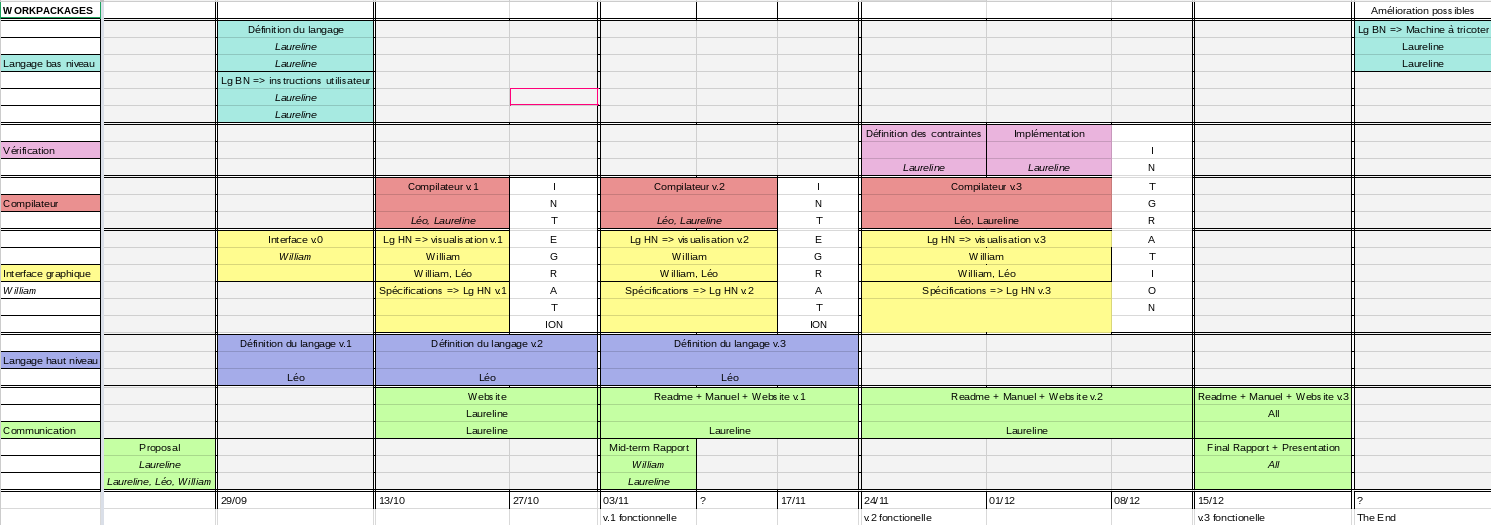
\includegraphics[scale=0.8,angle=270]{calendrier-previsionnel.png}
%  \includegraphics[scale=0.8]{calendrier-previsionnel-part1.png}
%  \includegraphics[scale=0.8]{calendrier-previsionnel-part2.png}
%  \caption{Calendrier prévisionnel des tâches}
%  \label{calendrier}
%\end{figure}

\newpage
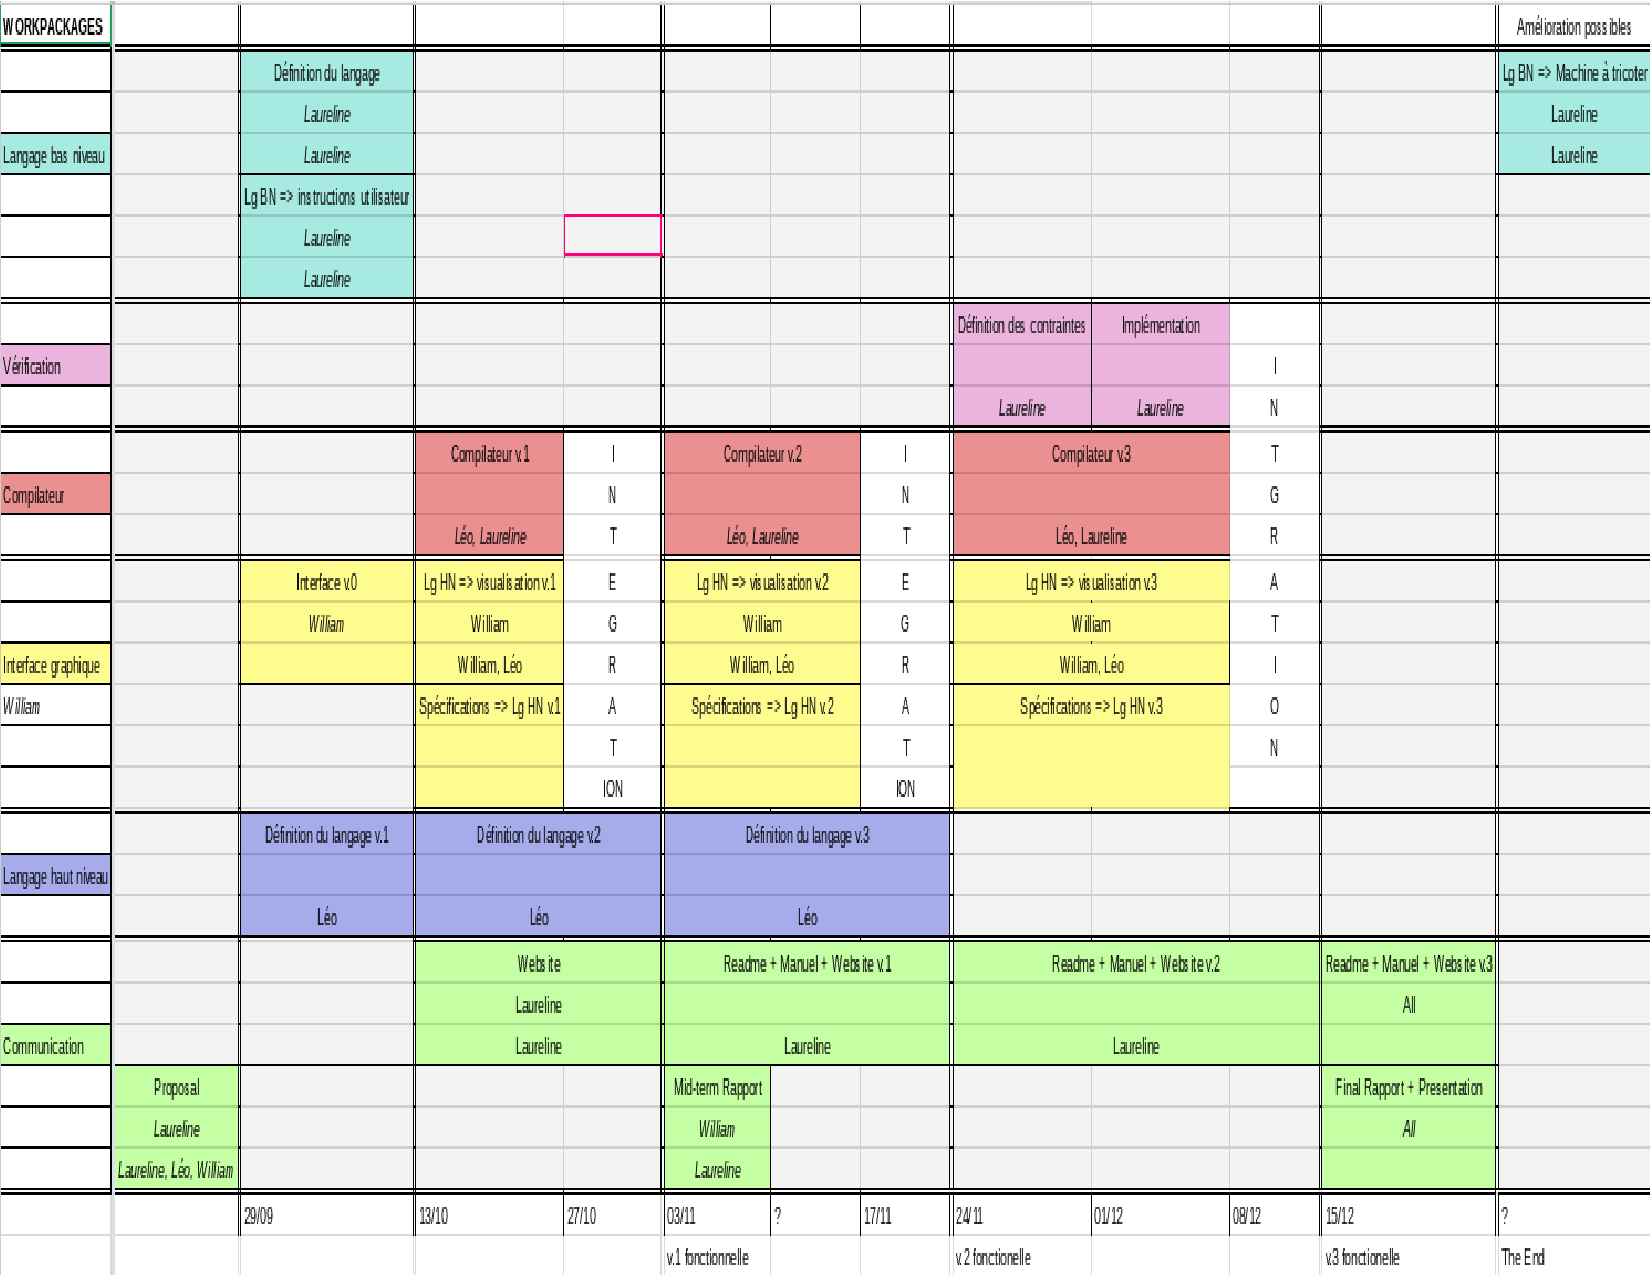
\includepdf{calendrier-previsionnel.pdf} %si on pouvait mettre la page en format paysage ce serait cool

% Calendrier à remplir

\end{document}
